\documentclass[10pt,xcolor=pdflatex,hyperref={unicode}]{beamer}
\usepackage{newcent}
\usepackage[utf8]{inputenc}
\usepackage[czech]{babel}
\usepackage[T1]{fontenc}
\usepackage{hyperref}
\usepackage{fancyvrb}
\usetheme{FIT}

\usepackage{algorithm2e}

%%%%%%%%%%%%%%%%%%%%%%%%%%%%%%%%%%%%%%%%%%%%%%%%%%%%%%%%%%%%%%%%%%
\title[Vázaný seznam]{Datové struktury\,--\,vázaný seznam}

\author[]{Michal Šmahel}

\institute[]{Fakulta informačních technologií
Vysokého učení technického v Brně\\
Bo\v{z}et\v{e}chova 1/2. 612 66 Brno -- Kr\'alovo Pole\\
xsmahe01@stud.fit.vutbr.cz}

\date{\today}
%%%%%%%%%%%%%%%%%%%%%%%%%%%%%%%%%%%%%%%%%%%%%%%%%%%%%%%%%%%%%%%%%%

\begin{document}

\section{Úvod}

\frame[plain]{\titlepage}

% \emph and \alert
\begin{frame}\frametitle{Proč využívat vázané seznamy?}
    \begin{itemize}
        \item Snadná implementace
        \item Jednoduché přidávání a mazání prvků
        \item Teoreticky neomezená velikost
        \item Nevyžadují spojitý blok paměti
        \item Obsahem může být libovolná datová struktura
    \end{itemize}
\end{frame}


\section{Vázaný seznam}

\begin{frame}\frametitle{Jednosměrně vázaný seznam}
    \begin{itemize}
        \item Dynamická datová struktura
        \item Složen z hlavičky a 0--$n$ položek
        \item \emph{Hlavička} odkazuje na první prvek seznamu
        \item Obsah \emph{položky} (jednosměrně vázaný):
            \begin{itemize}
                \item Uložená datová struktura
                \item Odkaz na další prvek seznamu
            \end{itemize}
    \end{itemize}
    
    \centerline{
\includegraphics[width=\textwidth]{img/linked-list-concept.png}}
\end{frame}

\begin{frame}\frametitle{Další typy vázaných seznamů}
    \begin{itemize}
        \item \emph{Dvousměrně} vázaný seznam
            \begin{itemize}
                \item Navíc odkaz na předchozí prvek
            \end{itemize}
    \end{itemize}
    
    \centerline{
\includegraphics[width=\textwidth]{img/doubly-linked-list-concept.png}}
    
    \pause
    
    \begin{itemize}
        \item \emph{Cyklický} vázaný seznam
            \begin{itemize}
                \item Speciální případ jednosměrného nebo dvousměrného
                \item Následník posledního prvku je první prvek
                \item Předchůdce prvního prvku je poslední prvek (dvousměrný)
            \end{itemize}
    \end{itemize}
    
    \centerline{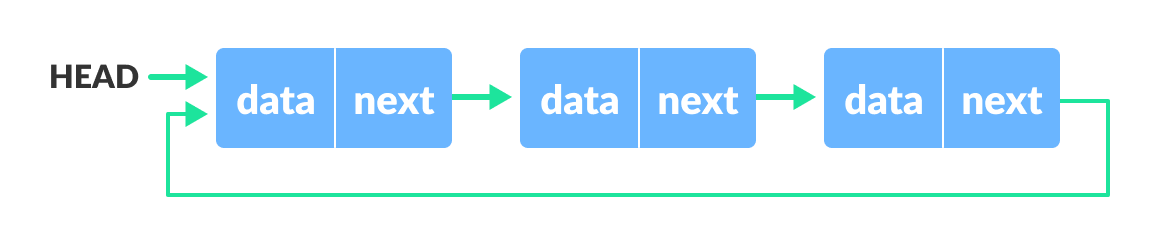
\includegraphics[width=\textwidth]{img/circular-linked-list.png}}
\end{frame}

\begin{frame}[fragile]\frametitle{Základní operace 1/4}
    \begin{itemize}
        \item \emph{Získání prvního} prvku
            \begin{itemize}
                \item Odkaz z hlavičky seznamu
                \item $O(1)$
            \end{itemize}
        
        \begin{algorithm}[H]
            % Solution of color \emph in algorithm
            \renewcommand{\emph}[1]{\textit{#1}}
    	    $item = HEAD \rightarrow first$\;
    	    $data = item \rightarrow data$\;
        \end{algorithm}
    \end{itemize}
\end{frame}

\begin{frame}[fragile]\frametitle{Základní operace 2/4}
    \begin{itemize}
        \item \emph{Přístup} k $n$-tému prvku
            \begin{itemize}
                \item Nutno projít všechny prvky od 1. do $n$-tého
                \item $O(n)$
            \end{itemize}
            
        \begin{algorithm}[H]
            % Solution of color \emph in algorithm
            \renewcommand{\emph}[1]{\textit{#1}}
            $item = HEAD \rightarrow first$\;
            $i = 0$\;
        	\While{$i$ < $n$}{
        	    $item = item \rightarrow next$\;
        	    $i = i + 1$\;
        	}
        	$data = item \rightarrow data$\;
        \end{algorithm}
    \end{itemize}
\end{frame}

\begin{frame}[fragile]\frametitle{Základní operace 3/4}
    \begin{itemize}
        \item \emph{Přidání} prvku na konec
            \begin{itemize}
                \item Vložení nového prvku do paměti
                \item Úprava odkazů (vložení do existujícího seznamu)
                \item $O(n)$
            \end{itemize}
        
        \begin{algorithm}[H]
            % Solution of color \emph in algorithm
            \renewcommand{\emph}[1]{\textit{#1}}
            $new\_item = \textbf{create } item$\;
            $last\_item = HEAD \rightarrow first$\;
        	\While{\textbf{exists} $last\_item \rightarrow next$}{
        	    $last\_item = last\_item \rightarrow next$\;
        	}
        	$last\_item \rightarrow next = new\_item$\;
        \end{algorithm}
    \end{itemize}
\end{frame}

\begin{frame}[fragile]\frametitle{Základní operace 4/4}
    \begin{itemize}
        \item \emph{Smazání} $n$-tého prvku
            \begin{itemize}
                \item Úprava odkazů (odebrání ze seznamu)
                \item Odstranění z paměti
                \item $O(n)$
            \end{itemize}
        
        \begin{algorithm}[H]
            % Solution of color \emph in algorithm
            \renewcommand{\emph}[1]{\textit{#1}}
            $item\_for\_delete = HEAD \rightarrow first$\;
            $i = 0$\;
        	\While{$i$ < $n$}{
        	    $previous\_item$ = $item\_for\_delete$\;
        	    $item\_for\_delete = item\_for\_delete \rightarrow next$\;
        	    $i = i + 1$\;
        	}
        	$previous\_item \rightarrow next = item\_for\_delete \rightarrow next$\;
        	\textbf{destroy} $item\_for\_delete$\;
        \end{algorithm}
    \end{itemize}
\end{frame}


\section{Závěr}

\bluepage{Děkuji za pozornost}

\begin{frame}[plain, noframenumbering]\frametitle{Použité zdroje}
    \begin{itemize}
        \item J. Řezáč: Příprava domácích úloh pro předmět Algoritmy. Brno, 2007. 52 s. Bakalářská práce. FIT VUT v Brně. Vedoucí práce B. Křena.
        \item T. Duda: Abstraktní datové typy pro jazyk C. Brno, 2007. 34 s. Bakalářská práce. FIT VUT v Brně. Vedoucí práce J. M. Honzík.
        \item Linked list\\
        \url{http://en.wikipedia.org/wiki/Linked_list}
    \end{itemize}
\end{frame}

\begin{frame}[plain, noframenumbering]\frametitle{Použité obrázky}
    \begin{itemize}
        \item Schéma jednosměrně vázaného seznamu\\
        \url{https://www.programiz.com/dsa/linked-list}
        \item Schéma dvojsměrně vázaného seznamu\\
        \url{https://www.programiz.com/dsa/linked-list-types}
        \item Schéma cyklického vázaného seznamu\\
        \url{https://www.programiz.com/dsa/linked-list-types}
    \end{itemize}
\end{frame}

\end{document}
